\section{\depsynth by Example}
\label{depsynth:s:overview}

This section illustrates the \depsynth development workflow
by walking through the implementation of a simple storage system.
We show how a developer can build a storage system with labeled writes
while assuming a strong crash consistency model,
and use \depsynth to automatically make that system crash consistent on real storage stacks.

\paragraph{Log-structured storage systems.}
A log-structured storage system
persists user data in a sequential log on disk~\cite{rosenblum:lfs}.
This design forsakes complex on-disk data structures
in favor of one with simple invariants and, as a result, simpler crash consistency requirements.
However, although log-structured storage systems are well studied,
their precise consistency requirements can be subtle
in the face of the caching and reordering optimizations used by the modern storage stack.

Consider implementing a simple key-value store as a log-structured storage system.
The on-disk data structure comprises two parts
as shown in \cref{fig:overview:layout}:
a log that stores key-value pairs (with one pair per block),
and a superblock that holds pointers to the head and tail of the log.
We will assume that single-block writes (\texttt{disk.write}) are atomic,
that each key-value pair fits in one block, 
and that the log does not run out of space.
To implement this system,
the developer writes \texttt{put} and \texttt{get} methods that interact with the disk:
%
\begin{lstlisting}[language=py]
class KeyValueStore(DepSynth):
  def __init__(self):
    self.superblock = disk.read(0)
    if self.superblock.empty():  # initialize an empty disk
      self.superblock_head, self.superblock_tail = 1, 1
    else:
      self.superblock_head, self.superblock_tail = from_block(superblock)
    self.epoch = 0

  def put(self, key: int, value: int):
    address = self.superblock_tail
    self.superblock_tail += 1

    new_block = to_block(key, value)
    disk.write(address, new_block, ("log", self.epoch))

    new_superblock = to_block(self.superblock_head, self.superblock_tail)
    disk.write(0, new_superblock, ("superblock", self.epoch))

    self.epoch += 1

  def get(self, key: int) -> Optional[int]:
    address = self.superblock_tail - 1
    while address >= self.superblock_head:
      block = disk.read(address)
      current_key, current_value = from_block(block)
      if current_key == key:
        return current_value
      address -= 1
    return None
\end{lstlisting}
%
Calls to \texttt{disk.read} and \texttt{disk.write} illustrate our new higher-level storage interface:
\texttt{disk.read} is unchanged from the usual system call,
taking as input an address on the disk to read from; and
\texttt{disk.write} takes as input an address on the disk to write to,
the block data to write to that address,
and a third \emph{label} argument.
A label is a pair of a string \emph{name} and an integer \emph{epoch}.
Labels serve as identities for writes:
the name describes the data structure the write targets,
while the epoch relates writes across different data structures.
This implementation uses the name part of the label to distinguish writes of new log blocks and writes to the superblock,%
\footnote{For this system we could distinguish the two data structures without labels---%
superblock writes are to address 0 while log writes are to non-zero addresses---%
but in general, storage systems reuse addresses over time and so this mapping is not static.}
and uses the epoch part as a logical clock
that relates the two writes generated by a single \texttt{put} call.
Labels exist only in memory while a write is in-flight,
and are never persisted to disk.

\begin{figure}
  \centering
  \begin{subfigure}[t]{0.48\textwidth}
    \centering
    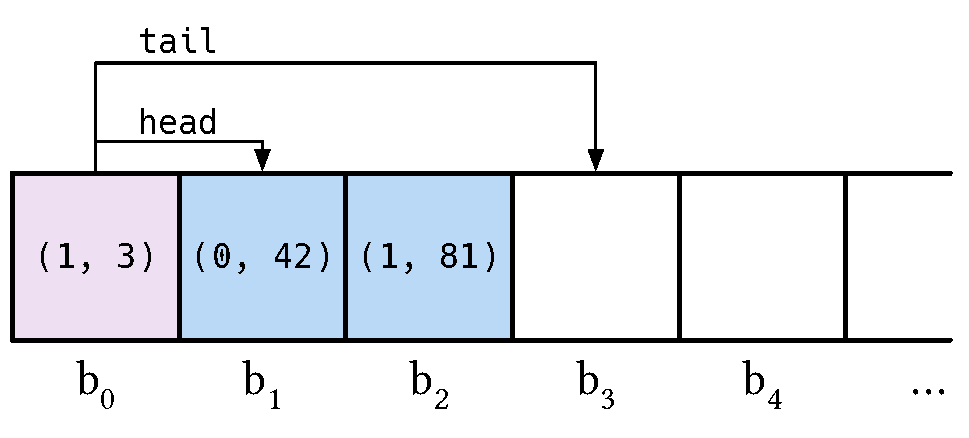
\includegraphics[width=0.8\textwidth]{figs/overview-good.pdf}
    \caption{On-disk layout of a simple log-structured key-value store. Each block holds a (key, value) pair.
    The first block is a superblock that holds pointers to the head and tail of the log.}
    \label{fig:overview:layout}
  \end{subfigure}%
  \quad%
  \begin{subfigure}[t]{0.48\textwidth}
    \centering
    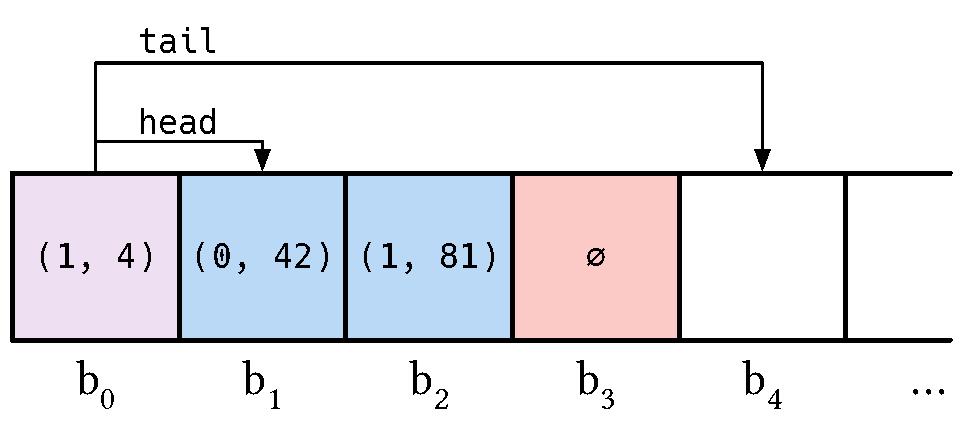
\includegraphics[width=0.8\textwidth]{figs/overview-crash.pdf}
    \caption{Possible on-disk state after a crash, leaving the superblock pointing to a range that includes an invalid block.}
    \label{fig:overview:crash}
  \end{subfigure}
  \caption{The on-disk layout of a simple key-value store. Arrows denote pointers and boxes are blocks.}
  \label{fig:overview}
\end{figure}

While this implementation is functionally correct,
it would not be crash consistent if implemented on a classical storage stack.
The issue is with the ordering of log and superblock writes:
even though the code suggests that the superblock write comes after the log write,
optimizations in the storage stack could reorder the two writes
and lead to a crash state where the superblock is updated but its corresponding new log block is not,
as \cref{fig:overview:crash} shows.
This would leave the \texttt{superblock_tail} pointer referring to an uninitialized disk block.
What we need for consistency is a way to preclude this reordering.
One solution in the \depsynth programming model
would be for the developer to manually implement a \emph{dependency rule}
that prevents this reordering:
%
\begin{lstlisting}[language=py]
  def __init__(self):
    self.rule("superblock", "log", eq)
\end{lstlisting}
%
A dependency rule \lstinline[language=py]{rule("a", "b", eq)}
specifies an ordering constraint:
a write labeled with name \lstinline[language=py]{"a"}
must not be sent to disk until after a write labeled with name \lstinline[language=py]{"b"}.
We say that such a rule means write \lstinline[language=py]{"a"} \emph{depends on} write \lstinline[language=py]{"b"},
or equivalently that write \lstinline[language=py]{"b"} must \emph{happen before} write \lstinline[language=py]{"a"}.
The third argument to \lstinline[language=py]{rule}
is an \emph{epoch predicate} that scopes the rule using the epoch in each label.
Here, the \lstinline[language=py]{eq} predicate
restricts the rule to only apply to pairs of writes whose labels have equal epochs.
% Throughout this paper, we use the notation $\deprule{a}{b}{p}$
% to denote a rule where a write labeled with name $a$ depends on a write labeled with name $b$ under epoch predicate $p$.
This rule means that superblock updates cannot be persisted on disk
until a log block write with the same epoch is persisted first,
ruling out the reordering behavior that could make the log inconsistent.\tighten

% While the developer could specify this dependency rule manually,
% our programming model does not require them to.
% Instead, \depsynth can automatically synthesize this rule, as described next.

\paragraph{Dependency rule synthesis.}
While the developer could specify the above dependency rule manually,
our programming model does not require them to,
and distilling the correct set of rules for a complex storage system is difficult to do by hand.
The challenge is a semantic gap:
the developer's desired high-level consistency property is about the on-disk data structure as a whole,
but the implementation of consistency can only refer to individual block-sized writes.
We bridge this gap with \depsynth, a program synthesis tool
that can \emph{automatically infer} the dependency rules sufficent to make a storage system crash consistent.

\depsynth takes three inputs.
First, it takes as input the implementation of the storage system.
Second, it takes as input a crash consistency predicate,
written as an executable checker over a disk state.
The crash consistency predicate
defines the property that should be true of \emph{every} state of the disk, 
including after crashes.
For our log-structured key-value store,
our desired consistency property is that the \texttt{superblock_tail} pointer
never gets ahead of the blocks that have been written to the log.
We can implement this property by checking that all blocks in the log are valid log blocks 
(we omit an implementation of \texttt{valid} for brevity,
but it could validate a checksum of the block):
%
\begin{lstlisting}[language=py]
  def consistent(self) -> bool:
    ret = True
    for address in range(self.superblock_head, self.superblock_tail):
      block = disk.read(address)
      ret = ret and valid(block)
    return ret
\end{lstlisting}
%
Finally, \depsynth takes as input a collection of \emph{litmus tests},
small programs that exercise the storage system.
Litmus tests are widely used to communicate the semantics of memory consistency models~\cite{alglave:litmus-tool,wickerson:memalloy},
and have also been used to communicate crash consistency models~\cite{bornholt:ferrite}.
A \depsynth litmus test comprises two executable programs \emph{initial} and \emph{main}.
Both programs take as input a reference to the storage system.
The \emph{initial} program sets up some initial state in the system, and cannot crash.
The \emph{main} program manipulates the system state, and can crash at any point.
For example, this is a simple litmus test that starts from a single log entry
and appends two more:
%
\begin{lstlisting}[language=py]
class SingleEntry_TwoAppend(LitmusTest):
  def initial(self, store: KeyValueStore):
    store.put(0, 42)
  
  def main(self, store: KeyValueStore):
    store.put(1, 81)
    store.put(2, 37)
\end{lstlisting}
%
As with previous work on memory consistency models~\cite{alglave:litmus-tool,bornholt:memsynth},
the developer can draw litmus tests from a number of sources:
they may be hand-written by the developer,
drawn from a common set of tests for important properties,
generated automatically by a fuzzer or program enumerator,
or intelligently generated by analyzing the on-disk data structures used by the storage system~\cite{alglave:diy}.

Given these three inputs,
\depsynth automatically synthesizes a set of dependency rules
that suffice to guarantee the crash-consistency predicate holds
on all crash states generated by all litmus tests.
For our example log-structured key-value store,
\depsynth synthesizes two dependency rules:
%
\begin{lstlisting}[language=py]
  def __init__(self):
    self.rule("superblock", "log", eq)
    self.rule("superblock", "superblock", gt)
\end{lstlisting}
%
The first rule is the same rule we hand-wrote earlier.
The second rule fixes a subtle crash-consistency bug in our hand-written implementation:
while the first rule ensures consistency for a \emph{single} put operation,
it still allows \texttt{superblock_tail} to get ahead of the log
if writes from \emph{multiple} puts are reordered with each other
(for example, reordering writes from the first and second puts in the litmus test above).
The second rule prevents this reordering using the \texttt{gt} epoch predicate,
which specifies that a superblock write with epoch $i$
cannot be persisted to disk until all superblock writes with lower epochs $j < i$ are persisted first.
The combination of these rules
precludes the problematic reordering
and guarantees that the superblock always refers to a valid \emph{range} of log blocks,
rather than only requiring the block at \texttt{superblock_tail} to be valid.
% Consistency failures in log writes similar to this one have caused data loss in the ext4 file system~\cite{gribincea:ubuntu-ext4}.

\if 0
\paragraph{Durability properties.}
We can also extend the \depsynth workflow to synthesize implementations
that satisfy stronger durability properties about a storage system.
For example, one durability property our log-structured key-value store should guarantee
is that once a key--value entry is persisted to disk,
it should never be lost by a subsequent crash.
To support such properties, crash consistency predicates in \depsynth
also accept an optional litmus test argument,
allowing them to refer to the expected state of the storage system:
%
\begin{lstlisting}[language=py]
  def consistent2(self, test: LitmusTest) -> bool:
    ret  = self.consistent()
    keys = test.expected_keys()
    for key in keys:
      ret = ret and self.get(key) != None
    return ret
\end{lstlisting}
%
The \texttt{expected_keys} method analyzes the litmus test statically to determine which keys
\emph{must} be present in any crash state of the key-value store.
For example, in the litmus test above,
we know that key \texttt{0} must be present as it is written by the initial method, which cannot crash.

\begin{figure}
  \centering
  \begin{subfigure}[t]{0.48\textwidth}
    \centering
    \includegraphics[width=0.8\textwidth]{example-image-golden}
    \caption{A crash state arising from reordering multiple puts.}
    \label{fig:overview2:put}
  \end{subfigure}%
  \quad%
  \begin{subfigure}[t]{0.48\textwidth}
    \centering
    \includegraphics[width=0.8\textwidth]{example-image-golden}
    \caption{A crash state arising from reordering during garbage collection.}
    \label{fig:overview2:gc}
  \end{subfigure}
  \caption{Two examples of crash-consistency violations that \depsynth can automatically rule out by inferring new dependency rules.}
  \label{fig:overview2}
\end{figure}

To see how this property might be violated,
consider adding garbage collection to the key-value store---%
if the same key is put into the store multiple times,
the previous entries are wasted space that can be reused
(although our toy implementation does not reuse blocks).
One naive garbage collection algorithm just iterates over all blocks in the log,
copies the entries that are still live,
and then moves the head of the journal:
%
\begin{lstlisting}[language=py]
  def garbage_collect(self):
    initial_tail = self.superblock.tail
    for address in range(self.superblock.head, initial_tail):
      block = disk.read(block)
      key, value = from_block(block)
      if value == self.get(key):
        self.put(key, value)
    self.superblock.head = initial_tail
    disk.write(0, to_block(self.superblock), ("superblock", self.counter))
    self.counter += 1
\end{lstlisting}
%
This garbage collection algorithm satisfies the original \texttt{consistent} predicate above,
because the range between the head and tail pointers always contains valid blocks.
But it can violate the durability property in \texttt{consistent2}:

% giving up here, not sure we need the extra detail.

\paragraph{Iterating on storage system design.}
\todo{not sure i need this part. but basically: let's add garbage collection to the log. it's hard and introduces new consistency issues,
but the synthesizer takes care of those automatically. use this to demonstrate ``initial state'' of a litmus test,
to speciofy durability properties.}

\fi

\if 0

\depsynth is a tool for adding crash consistency code to storage systems.
To use \depsynth, developers provide a base system implementation, a crash
consistency property, and a set of example programs that can run over their system.
In this section, we show the design process of a crash consistent system using
\depsynth and how developers use the output of \depsynth.
\todo{make a figure for the input/output behavior of \depsynth?}

\paragraph{A simple key-value store}
\todo{Better transition here? Outline this subsection?}
We start with the design of a simple key-value store that inserts data with \putreq requests,
retrieves data with \get requests, and flushes data to disk with \flush requests.
These requests are synchronous, and in general, \depsynth does not support concurrency.
Our disk model allows the operations \texttt{(read! region location length)},
\texttt{(write! region data location)}, and \texttt{(flush! region)}, which read (possibly cached)
data from disk, write data to disk, and flush data to disk respectively. The disk also allows \texttt{(append! region data)},
which is the same as a \texttt{write!} to the end of the disk region. \texttt{flush!} is important because
writes to disk are not immediately committed, meaning that the write data may still be in a buffer and not
yet actually on the disk. After \texttt{(flush! region)}, all writes to disk region \texttt{region} are committed.
Additionally, data from \texttt{write!} or \texttt{append!} is formatted into one or more pages, and flushing
each page to disk is done atomically. There are no assumptions made about the state of the disk before
a program (i.e. sequence of \putreq, \get, \flush) is run.

One way to design a key-value store is to store metadata and data separately \todo{cite, wisckey, shardstore}.
This allows the implementation of \get to avoid scanning through all of the stored data.
On disk, one region is reserved for an index of metadata, and another region is reserved for
a store of data. On request $\putreq\ K\ V$, our implementation appends the metadata $(K, L, |V|)$
to the index and the data $V$ to the store, where $L$ is the location of $V$
in the store disk region. An implementation of this design is shown in \autoref{fig:kv-single-index}.

\todo{Should probably change code to be imperative/pythonic}

\begin{figure}[h]
  \centering
  \resizebox{\linewidth}{!}{%
    \begin{minipage}{1.03\linewidth}
      \lstinputlisting[language=rosette,xleftmargin=-.5em,firstline=1,basicstyle=\scriptsize\ttfamily]{code/kv-single-index.rkt}
    \end{minipage}}
  \vspace{-.5em}
  \caption{Implementation of a key-value store with a separate metadata index}
  \label{fig:kv-single-index}
\end{figure}

\paragraph{What can go wrong?}
Recall that writes from \texttt{append!} can be buffered by the disk and committed later.
Suppose a user of our key-value store issues a request $\putreq\ '\texttt{a}' \ 7$.
Our implementation would write $('\texttt{a}', 0, 1)$ to the index and $(7)$ to the data store, both of which are
buffered. Since the disk can choose the order of these writes to commit, it chooses to commit
$('\texttt{a}', 0, 1)$ to the index first. Then, before the disk is able to commit $(7)$ to the data store, the
power goes out and the disk crashes. Upon booting back up, the index data is on disk but the actual data $(7)$ is not.
This means that any future requests $\get\ '\texttt{a}'$ could return incorrect data. This is especially bad
because from a users perspective, there is no notification of an error in our system.
\todo{Make figure that shows (old and new) behavior of $\get\ '\texttt{a}'$}

\paragraph{How can we fix this problem?}
There are several ways that storage systems can ensure the crash consistency of their data.
Journaling, copy-on-write, and soft updates are among the most popular ways that systems
implement crash consistency \todo{cite}. In this paper, we focus on implementing crash consistency
with soft updates. Soft updates work by specifying a partial order over disk writes that restricts
when writes can be committed to disk. FeatherStitch \todo{cite} showed that these restrictions can be
specified as dependencies or "write-before" relationships between disk writes, where the relationship
``$A$ depends on $B$'' means that $A$ should only be sent to disk after $B$ is committed on disk.
If we treat these relations as directed edges between disk writes, we get a \textit{dependency graph}.
To fix our example with soft updates, we could make the index write \textit{depend on} the data write.
Then, after any crash, $\get\ '\texttt{a}'$ would either return \texttt{false} (when not all data is committed
before the crash) or the correct value: $7$.

\depsynth generates crash consistency code using the soft updates model.
This gives storage systems built with \depsynth the advantage of faster performance because unlike
other methods of implementing crash consistency, soft updates avoids duplicating writes.
Specifically, \depsynth outputs a set of \textit{rules} that specify how to construct dependencies
between disk writes emitted by the storage system.

\paragraph{Crash Consistency Properties and Dependency Rules}
Now we can discuss precisely what crash consistency means for our basic key-value store. When a disk
crash occurs and later reboots, future calls to $\get\ K$ should either report a failure or should
return some value $V$ where some $\putreq\ K\ V$ was issued before the crash. $\get\ K$ should only
report a failure when the data and metadata for $K$ had not been completely committed before the crash
Concretely, we can encode this crash consistency property by maintaining a reference model that
describes all possible crash consistent behaviors for any sequence of operations on our key-value store.

\todo{make a figure for the reference model and crash consistency property?}

The only way that this property can be broken in our simple key-value store is in the case we previously
discussed: a crash happens after an index write is committed and before the corresponding data write is committed.
As we mentioned, we can avoid this situation by making the index write \textit{depend on} the data write.
In fact, each pair of writes from a \putreq request should have this relationship. \depsynth encodes this fact
as a \textit{dependency rule}, which is a tuple of \textit{parent label}, \textit{child label},
and \textit{timing relation}.
For example, consider the rule that \depsynth outputs for our simple key-value store:

%$$ \texttt{put:append!(index)} \rightarrow_= \texttt{put:append!(data-store)} $$
$$ \deprule{\texttt{put:append!(index)}}{\texttt{put:append!(data-store)}}{=}$$

Here, the parent label is \texttt{put:append(index)}, the child label is \texttt{put:append(data-store)},
and the timing relation is $=$. Parent and child labels match individual disk writes issued by the
system implementation. In this case, the parent would be any write to the index from an \texttt{append!} in the
\texttt{put} function implementation, while the child would be any write to the data store from an \texttt{append!}
in the \texttt{put} implementation. The timing relation specifies if the rule should apply within a single request
or across requests. Here, the timing relation $=$ specifies that the rule should only apply to writes that were
generated by the same \putreq request.

\paragraph{Automatically generating crash consistency rules}
Writing dependency rules requires reasoning about disk states in the presence of a crash, which can
be difficult to do as the complexity of a system increases. \depsynth is a tool for automatically
synthesizing dependency rules, removing this burden from the developer. As input, \depsynth takes
the implementation of the storage system along with the crash consistency property and a set of
example sequences of operations over the system. We call these sequences of operations
\textit{litmus tests}, inspired by work in memory consistency models \todo{cite, ferrite, memory models}.
A set of three litmus tests for our basic key-value store is shown in \autoref{fig:test-set}.
An important point about litmus tests is that when checking for correctness with respect to the crash consistency
property, we only consider crashes that occur during flush points (i.e. whenever \texttt{flush} is called on
a disk region and at the end of the test). This is sufficient because crashing at any
other point has the same affect on the disk state as crashing at the end of the most recent flush.
\todo{I'm not totally sure how to explain this briefly. I think the term "flush point" comes out of nowhere and seems random.}
With these three inputs, \depsynth outputs the dependency rule shown previously.

\begin{figure}[h]
  \centering
  \resizebox{\linewidth}{!}{%
    \begin{minipage}{1.03\linewidth}
      \lstinputlisting[language=rosette,xleftmargin=-.5em,firstline=1,basicstyle=\scriptsize\ttfamily]{code/test-set.rkt}
    \end{minipage}}
  \vspace{-.5em}
  \caption{Set of example requests for our key-value store}
  \label{fig:test-set}
\end{figure}

As the complexity of our system and of crash behaviors increases, determining
correct ordering rules becomes more difficult for developers.
To demonstrate this point, we improve upon the previous key-value store design by improving
space efficiency in the index. The amount of space used by the index was dependent on the number of \putreq
requests in the old design. This new design will improve upon this, making the size of the index instead
dependent on the number of keys stored. We can do this by adding a \clean operation which removes
all overwritten metadata from the index.

\begin{figure}[h]
  \centering
  \resizebox{\linewidth}{!}{%
    \begin{minipage}{1.03\linewidth}
      \lstinputlisting[language=rosette,xleftmargin=-.5em,firstline=1,basicstyle=\scriptsize\ttfamily]{code/kv-wrong-index.rkt}
    \end{minipage}}
  \vspace{-.5em}
  \caption{Naive implementation of a key-value store with \clean}
  \label{fig:kv-wrong-index}
\end{figure}

A naive new implementation for \clean would read the index, remove overwritten metadata for all keys that
appear more than once, and write the result back out to the index as seen in \autoref{fig:kv-wrong-index}.
After updating the implementation and litmus test set and running \depsynth again, we get the following result:
\texttt{No rules found}.

This means that \depsynth was unable to find a set of rules that guarantees our crash consistency
property under all crash behaviors. \depsynth also outputs the litmus test that caused it to fail,
shown in \autoref{fig:failing-test}. To help understand what went wrong, the state of the data store
and index after each request is shown in a comment. The data within \texttt{*...*} has been flushed to disk.
\todo{This is not something that's output by \depsynth, I just put it here to help explain what's going on. I could make \depsynth output it though, but that seems like a minute implementation detail}

\begin{figure}[h]
  \centering
  \resizebox{\linewidth}{!}{%
    \begin{minipage}{1.03\linewidth}
      \lstinputlisting[language=rosette,xleftmargin=-.5em,firstline=1,basicstyle=\scriptsize\ttfamily]{code/failing-test.rkt}
    \end{minipage}}
  \vspace{-.5em}
  \caption{Test that causes \depsynth to return \texttt{No rules found}}
  \label{fig:failing-test}
\end{figure}

Recall that while single writes $(K, L, |V|)$ to the index are atomic (since it fits in a page),
writing the entire contents of the index is not. Consider a crash that occurs after the test case in
\autoref{fig:failing-test}, before all data is committed to disk. Since the crash happens while the
index is being updated from \clean, previous entries could be incompletely overwritten. Metadata that
was completely flushed to disk by \flush could be lost, breaking our crash consistency property.
This is exactly the behavior in \autoref{fig:failing-test} that causes \depsynth to fail.

Understanding this, we can adjust the design of our key-value store to avoid overwriting old entries
and make crash consistency possible. Instead of writing the updated index to the same disk region,
our key-value store will keep two distinct regions, alternating between them when updating the
index. Additionally, our key-value store needs to reserve a distinct block to update the pointer
indicating the current set of index region being used. On a \clean operation, we read the old index
and remove outdated metadata, but instead of writing to the same index region, we update the index
pointer and write the updated index metadata to the previously unused index region. Our new
implementation is shown in \autoref{fig:kv-double-index}.

\begin{figure}[h]
  \centering
  \resizebox{\linewidth}{!}{%
    \begin{minipage}{1.03\linewidth}
      \lstinputlisting[language=rosette,xleftmargin=-.5em,firstline=1,basicstyle=\scriptsize\ttfamily]{code/kv-double-index.rkt}
    \end{minipage}}
  \vspace{-.5em}
  \caption{Implementation of a key-value store design with \clean}
  \label{fig:kv-double-index}
\end{figure}

With this updated key-value store implementation, we can run \depsynth again to find a new set of
rules that ensure our crash consistency property holds. \depsynth outputs the following new rules.

\begin{align*}
  \texttt{put:append!(index)} &\rightsquigarrow_= \texttt{put:append!(data-store)} \\
  \texttt{clean:update!(index-pointer)} &\rightsquigarrow_= \texttt{clean:append!(data-store)} \\
  \texttt{clean:update!(index-pointer)} &\rightsquigarrow_> \texttt{put:append!(data-store)}
\end{align*}

The first rule is the same as the rule from our simpler example.
The second rule states that the update to the index pointer should wait until the updated
index metadata has been written. Without this rule, a crash could allow the index pointer
to be updated to an old (and possibly empty) version of the index.
The third rule states a stronger requirement: that the update to the index pointer should
wait until \emph{all} writes to the data store from previous \putreq requests have completed.\tighten

\fi
